\documentclass[a4paper,12pt,twoside,BCOR=10mm]{scrbook}

% Packages
\usepackage{ucs}
\usepackage[utf8x]{inputenc}
\usepackage[icelandic, english]{babel}
\usepackage{t1enc}
\usepackage{graphicx}
\usepackage[intoc]{nomencl}
\usepackage{enumerate,color}
\usepackage{url}
\usepackage[pdfborder={0 0 0}]{hyperref}
\usepackage{appendix}
\usepackage{eso-pic}
\usepackage{amsmath}
\usepackage{amssymb}
\usepackage[nottoc]{tocbibind}
\usepackage[sort&compress,authoryear]{natbib}
\usepackage[sf,normalsize]{subfigure}
\usepackage[format=plain,labelformat=simple,labelsep=colon]{caption}
\usepackage{placeins}
\usepackage{tabularx}
\usepackage{wrapfig}
\usepackage{courier}
% Configurations
\graphicspath{{img/}{../img/}}

\setlength{\parskip}{\baselineskip}
\setlength{\parindent}{0cm}
\raggedbottom
% \setkomafont{subsection}{\normalfont\sffamily}

% Eins og templatið á að vera
% \setkomafont{captionlabel}{\itshape}
% \setkomafont{caption}{\itshape}

% Mun fallegri lausn
\setkomafont{captionlabel}{\itshape}
\setkomafont{caption}{\itshape}
\setkomafont{section}{\FloatBarrier\Large}
\setcapwidth[l]{\textwidth}
\setcapindent{1em}


% Times new roman
%\usepackage[T1]{fontenc}
%\usepackage{mathptmx}

%%%%%%%%%%% MODIFY THESE LINES ONLY %%%%%%%%%%%%%%%%%%%%%%%%%%%%%%%%%%%%%%%%%%%%%%%%%%%%%%%%%
\def\thesisyear{2013}       						% Year thesis submitted
\def\thesismonth{October}						% Month thesis submitted
\def\thesisauthor{Baldur Þór Emilsson}					% Thesis authoreiningaraðferðinni
\def\thesistitle{Marty: Application Development and Testing with Production Data in PostgreSQL} % Title of thesis
\def\thesisshorttitle{Development and Testing with Production Data} 	% Title of thesis
\def\thesiscredits{60} 							% Credits awarded for the project
\def\thesissubject{Computer Science}
\def\thesiskind{M.Sc.}							% Masters of PhD thesis
\def\thesiskindformal{Magister Scientiarum}				% Masters of PhD thesis
\def\thesisnroftutors{1}						% Number of tutors
\def\thesisschool{School of Engineering and {Natural Sciences}}		% School
\def\thesisfaculty{Industrial Engineering,\\Mechanical Engineering and\\Computer Science} % Faculty
\def\thesisaddress{Hjarðarhaga 2-6}					% Office address
\def\thesispostalcode{107, Reykjavik}					% Office address
\def\thesistelephone{525 4700}						% Office telephone
\def\thesistutors{Hjálmtýr Hafsteinsson}
\def\thesisrepresentative{XXNN3}					% Tutors name
\def\thesisPrinting{Háskólaprent, Fálkagata 2, 107 Reykjavík}

% Function to add footer to frontpage
\newcommand\BackgroundPic{
\put(0,0){
\parbox[b][\paperheight]{\paperwidth}{
\vfill
\centering
\hspace*{-0.6cm}

\includegraphics[width=\paperwidth,height=\paperheight,
keepaspectratio]{foot}
}}
\setlength{\unitlength}{\paperwidth}
\begin{picture}(0,0)(0,-0.15)
\put(0,0){\color{white}\parbox{1\paperwidth}{\centering\bfseries\sffamily \Large Faculty of \thesisfaculty \\
University of Iceland\\
\thesisyear}}
\end{picture}
}

\begin{document}

\begin{titlepage}
\thispagestyle{empty}
\AddToShipoutPicture*{\BackgroundPic}
%
\begin{center}
\vspace*{1cm}

\includegraphics[width=43.6mm]{ui_1_cmyk}\\
\vspace*{3.0cm}
\huge \sffamily \bfseries \thesistitle

\vspace*{5.5cm}
\normalfont \Large \sffamily \thesisauthor
\AddToShipoutPicture*{\BackgroundPic}
\vfill

\end{center}

\newpage 
\thispagestyle{empty} \mbox{}
\newpage
\vspace*{1.35cm}
\thispagestyle{empty}
\begin{center}

\Large \textbf{\sffamily{\MakeUppercase{\thesistitle}}} \\

\vspace*{1.7cm}
\sffamily{\thesisauthor} \\
\vspace*{1.8cm}
\normalsize \thesiscredits~ECTS thesis submitted in partial fulfillment of a \\
\textit{\thesiskindformal} degree in \thesissubject

\vspace*{1.0cm}
\large
\ifnum\thesisnroftutors >1 Advisors \\ \thesistutors \\ \vspace*{0.4cm}
\else Advisor \\ \thesistutors \\ \vspace*{1.04cm}
\fi
Faculty Representative \\
\thesisrepresentative

\vfill
Faculty of \thesisfaculty \\
\thesisschool \\
University of Iceland \\
Reykjavik, \thesismonth~\thesisyear
\newpage
\end{center}
 \newpage
 \thispagestyle{empty}
 \mbox{} \vfill
 % \setcounter{page}{0} \renewcommand{\baselinestretch}{1.5}\normalsize
 \sffamily{\thesistitle} \\
 \sffamily{\thesisshorttitle} \\
 \thesiscredits ~ECTS thesis submitted in partial fulfillment of a \thesiskind~degree in \thesissubject
\\ \\
Copyright \textcopyright~\thesisyear~ \thesisauthor \\
All rights reserved \\


Faculty of \thesisfaculty \\
\thesisschool \\
University of Iceland \\
\thesisaddress \\
\thesispostalcode, Reykjavik \\
Iceland

Telephone: \thesistelephone \\ \\
\vspace*{\lineskip}

Bibliographic information: \\
\thesisauthor, \thesisyear, \thesistitle, \thesiskind~thesis, Faculty of \thesisfaculty, University of Iceland. \\

Printing: \thesisPrinting \\
Reykjavik, Iceland, \thesismonth~\thesisyear \\
\newpage
\end{titlepage}


\pagenumbering{roman}

\setcounter{page}{3}
\section*{\huge Abstract}
Marty is a proof-of-concept prototype for a framework that offers convenient application development and testing against data used in production that is stored in the PostgreSQL database management system.
It is designed for minimal overhead and configuration on production servers while offering quick and simple database initialization on development and testing servers.
This opens the possibility for application testing on production data with minimal effort, which complements conventional testing datasets and helps preventing bugs from entering production code which were not caught with the conventional datasets.
\vfill \vspace*{1cm}
\section*{\huge Útdráttur}
Marty er hugbúnaðarlausn sem býður upp á þægilegt þróunar- og prófunarumhverfi fyrir forrit sem nota PostgreSQL gagnagrunnskerfið.
Hún er hönnuð til að nota gögn úr gagnagrunnum sem keyra í raunumhverfi án þess að hafa neikvæð áhrif á afköst netþjónanna sem grunnarnir keyra á og án mikilla breytinga á uppsetningu þeirra en bjóða á sama tíma upp á fljótlega og einfalda uppsetningu þróunar- og prófunargagnagrunna.
Það opnar fyrir möguleikann á hugbúnaðaprófunum með raungögnum án mikillar fyrirhafnar sem geta keyrt samhliða prófunum með hefðbundin prófunargagnasett og hjálpað við að uppræta villur sem koma ekki í ljós með hefðbundnum prófunum.
\vfill
\newpage

\tableofcontents
\listoffigures
\listoftables

\chapter*{Abbreviations}
\addcontentsline{toc}{chapter}{Abbreviations}
Í þessum kafla mega koma fram listar yfir skammstafanir og/eða breytuheiti. Gefið kaflanum nafn við hæfi, t.d. Skammstafanir eða Breytuheiti. Þessum kafla má sleppa ef hans er ekki þörf. \\

The section could be titled: Glossary, Variable Names, etc.

\chapter*{Acknowledgments}
\addcontentsline{toc}{chapter}{Acknowledgments}
Í þessum kafla koma fram þakkir til þeirra sem hafa styrkt rannsóknina með fjárframlögum, aðstöðu eða vinnu. T.d. styrktarsjóðir, fyrirtæki, leiðbeinendur, og aðrir aðilar sem hafa á einhvern hátt aðstoðað við gerð verkefnisins, þ.m.t. vinir og fjölskylda ef við á. Þakkir byrja á oddatölusíðu (hægri síðu).

\chapter{Introduction}
\pagenumbering{arabic}
\setcounter{page}{1}
Database management systems (DBMS) are used as datastores in many different systems in various fields.
They are rarely used as standalone products and are usually used to store data from other applications.
These applications are often in constant development with short development cycles, which include both manual and automated testing.
Those  tests are often run against datasets that are created to test for specific conditions and ideally they help with catching all bugs before they enter production. However, many projects can benefit from tests that are run against data from the production environment, either to complement the testing datasets or to provide data to test against in situations where no testing datasets exist.
The main disadvantage of using production data in testing is that cloning a large database can take a long time which slows down testing and development and it adds an overhead to the database in production which can have negative effects on the performance of the application in the production environment.

The goal of Marty is to offer a convenient and relatively efficient way to run tests for applications that use the PostgreSQL (Postgres) DBMS against the live data on the production servers without adding overhead to them.
This is achieved by creating a testing database with empty tables that are populated  when they are first queried.
This saves time as only the tables which are used in the tests are populated and no time is spent copying the data for the other tables, which remain empty.
The data is not copied directly from the production server but from another instance of Postgres that stores a copy of the production data.
This is done to ensure the consistency of the data in the cloned databases and also to minimize the load on the production database.
A byproduct of this architecture is the possibility to inspect the state of the production database as it was at a certain point in time.

% TODO rewrite this section when the thesis is complete: The rest of this thesis is organized as follows: chapter 2 contains details about the history of Postgres and its internals that are relevant to Marty. In chapter 3 the design of Marty is described along with reasoning for why this design was chosen and some details about the implementation of Marty. The fourth and final chapter contains conclusions and future work.

\section{Goals and purpose of Marty}
The goal of the development of Marty is to create an application that enables its users to clone a running database quickly.
The original idea was that software developers and testers would be able to clone a database that is used in production and stores large amounts of data that would normally take a considerable time to copy to another server.
Marty will speed up development and testing by reducing the time it takes to clone the production database and also uses techniques that reduce or prevent any negative impact that the cloning would have on the performance of the production database. 

Although the initial idea was for production databases to be cloned there is nothing that prevents Marty to be used for other kinds of databases, such as databases that are dedicated to storing test datasets that never enter production, as long as those databases fulfill the requirements for Marty.

The emphasis in the design and development of Marty is to minimize the time from when the cloning of a database is initialized and until the newly created clone can be used for testing.
The performance of the newly created database has not been a high priority as it is not intended to be used in a performance critical environment.
Thus Marty is not a solution that should be used to create clones of a database that are to be used for load balancing or failover or serve any other role in the production environment of an application.

Marty is supposed to be used in an environment where a one or a few databases need to be cloned regularly.
The architecture that was chosen for Marty requires a system administrator to set up and configure Marty for the environment where it is used.
This involves running a dedicated Postgres instance that is used as a reference when the clones are created and also configuring the production server to work with this dedicated instance in a certain way, which might require the production server to be restarted.
It should therefore be clear that Marty is not suited for cloning a database that only needs to be cloned for a limited number of times.
It should be most useful when the database to be cloned is large enough that the time saved by using Marty justifies the initial setup.

\chapter{Architecture}
This chapter contains a detailed description of the architecture and design of Marty.

\section{Overview}
Marty consists of a few parts that serve different pruposes, see figure \ref{architecture-overview}.
Developers and testers that use Marty in their work create database \textit{clones}.
These databases are clones of the \textit{master} database, which can be a database that is used in a production environment.
When the clones are created they are initialized with a copy of all the tables in the master, but the tables remain empty until they are queried by a user or an application.
The design of the clone databases is discuessed in chapter \ref{sec:clones}.

\begin{figure}[h!]
  \centering
    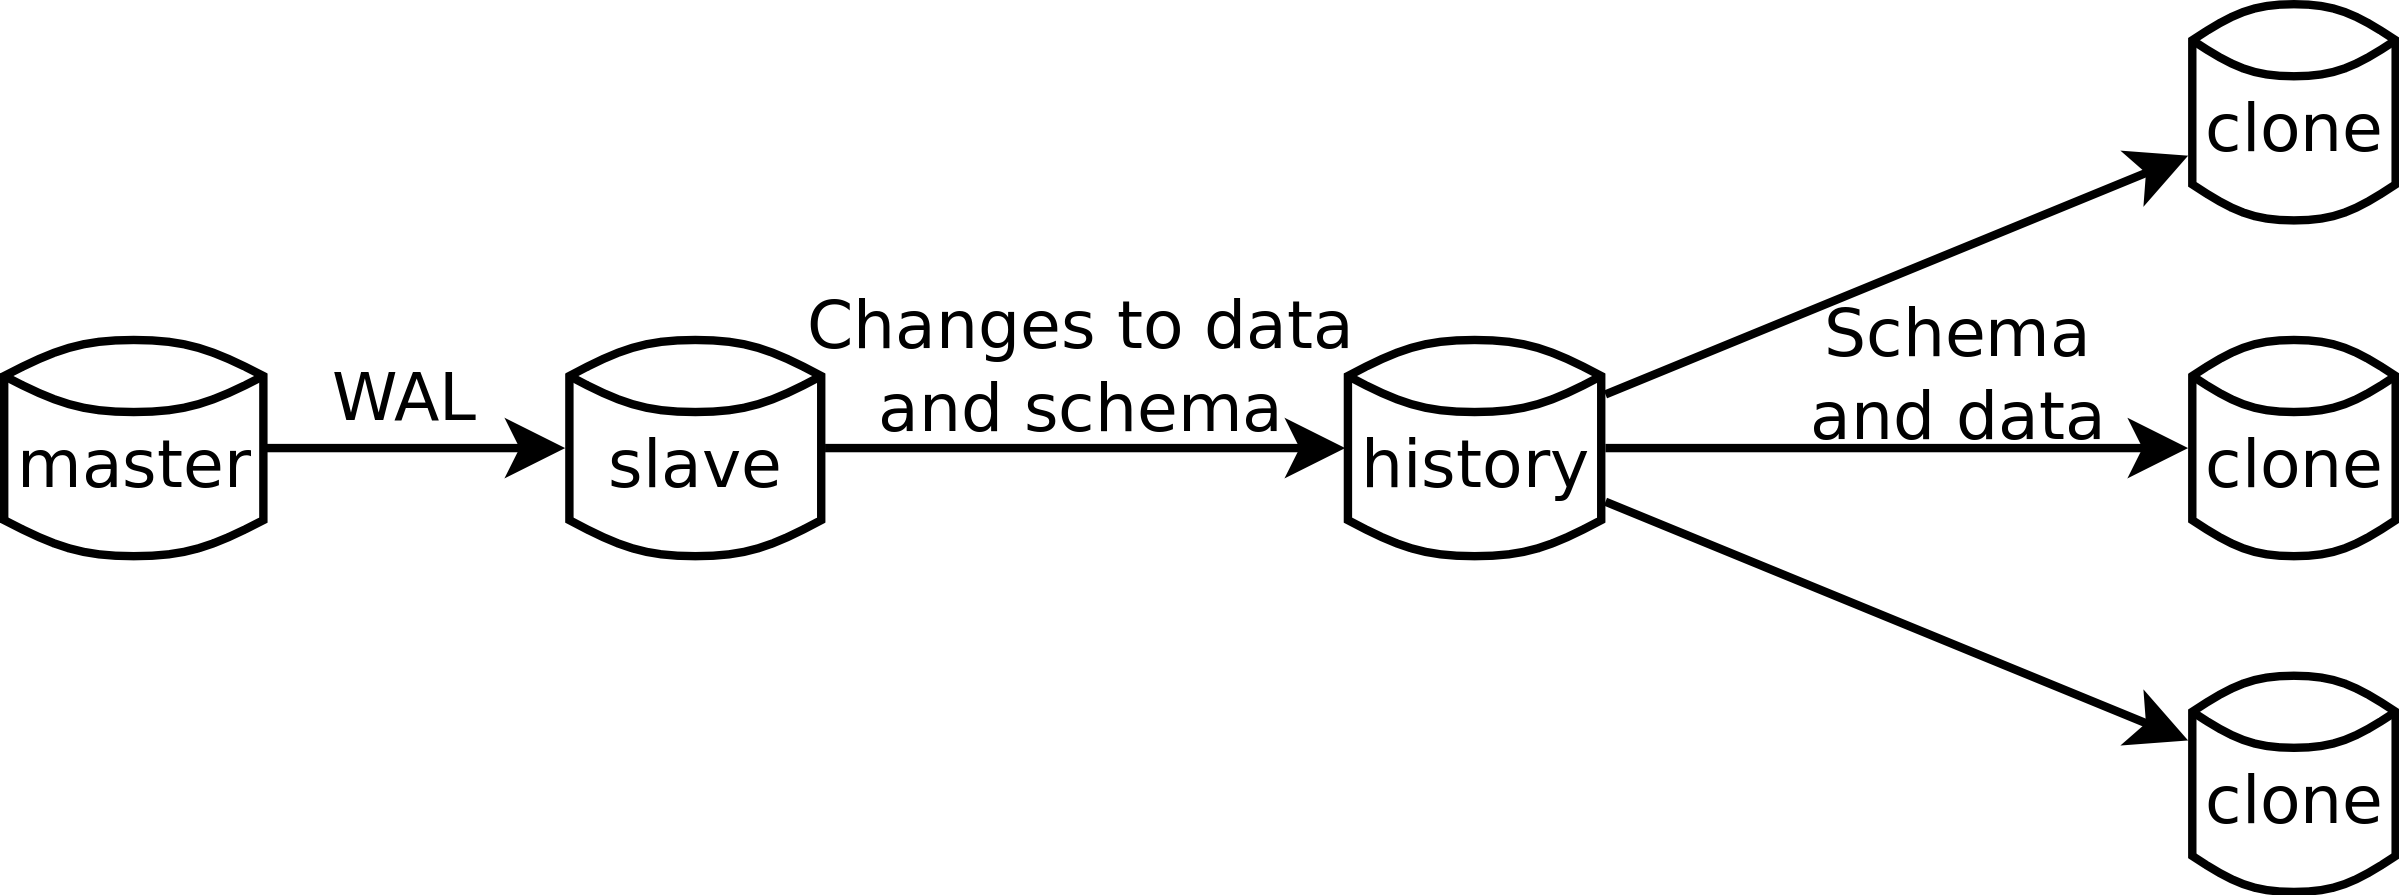
\includegraphics[width=0.8\textwidth]{architecture}
  \caption{An overview of the architecture of Marty}
  \label{architecture-overview}
\end{figure}

Marty does not inspect the schema of the master database directly when it creates the tabes in the clone databases.
Instead it queries another database that is called \textit{history}.
The history database contains information about the schema of the master database as well as a copy of its data.
When the clones need to populate their tables they also use this history database as a reference.
The reason for using another database to store a copy of the schema and data of the master database is discussed in chapter TODO, along with a description of the design of the history database.

As the name suggests the history database contains not only a copy of the current version of the master but also of previous versions.
To update the history database with new versions of the master and to keep it in sync with the changes that are made on the master Marty uses a log from the master that is called the \textit{write-ahead log} or \textit{WAL}.
It does not read this log directly but uses a specially patched instance of Postgres to read the contents of the log.
This instance is called \textit{slave} and it outputs information that Marty can use to update the history database with all the changes that have been made in the master database.
The reason for keeping old versions of the master database and the relationship between the master, slave and history databases is described in detail in chapter TODO.

\section{The clone databases}
\label{sec:clones}
A clone database is a standard Postgres database.
It uses two Postgres extensions; the \textit{PL/pgSQL} extension that enables users to create stored procedures, and the \textit{dblink} extension which enables users to query another database directly from the clone database without using any external scripts or programs.
The clone can run on a local instance of Postgres on the developers' or testers' computer as long as the history database is accessible from that computer.
More than one clone database can run in parallel on the same instance of Postgres so each user can use many clones at the same time.

To create a clone the user creates a new, empty database.
She then initializes it with Marty.
After the clone has been initialized it contains all the schemas that are found in the master database and a copy of all the tables from each schema.
The tables remain empty until they are first queried which saves time in the initialization as the user does not have to wait for Marty to finish copying all the data in the tables before she can start querying the clone.
This behaviour is implemented by creating views instead of tables in the clone.
The views look like the tables that the user expects to find and when they are queried they call a PL/pgSQL function, \textit{view\_select}, that returns the appropriate data.
This function looks for the data in the actual data tables, which Marty creates in the clone, and if these tables are empty the function populates them with data from the history database before returning their contents.

The data tables are created in a special schema called \textit{marty} which is created in the clone database.
It contains the data tables as well as another table called bookkeeping.
The view\_select function uses this table to keep track of which data tables have been populated and which ones are still unpopulated.
The table also contains the querystrings that view\_select uses when it fetches the data from the history database.
See figure \ref{clone-architecture} for an example of a table layout in a clone database.

The views, bookkeeping table, data tables and the view\_select function are described in detail in chapter TODO.

\begin{figure}[h!]
  \centering
    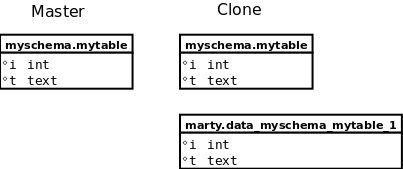
\includegraphics[width=0.5\textwidth]{clone-architecture}
  \caption{Table layout in a clone database}
  \medskip
  \small
  The table \textit{mytable} is actually a view that returns results from the table \textit{data\_myschema\_mytable\_1} which is in the \textit{marty} schema.
  \label{clone-architecture}
\end{figure}

\section{The history database}
The history database is a standard Postgres database.
It is created by a system administrator and contains data that the developers and testers use when they create clone databases.
When the history database has been initialized it contains information about the schema of the master database and a copy of its data.
After the initialization Marty updates the history database with all the changes that are made in the master, both to its data and schema.
Its contents are versioned and, as the name suggests, the user can look up previous states of the master in the history database.

The reason for keeping old versions of the master is the delayed population of the data tables in the clones.
From the moment that a clone database is initialized and until its tables are populated the master database might change.
Tables might be dropped or renamed and rows might be updated or deleted, which could lead to inconsistency in the clone as foreign key relations might break.
The history database offers access to a particular version of the contents of the master database and thus prevents errors of this kind in the clones.

Marty initializes the history database with four tables; \textit{marty\_schemas}, \textit{marty\_tables}, \textit{marty\_columns} and \textit{marty\_updates}.
The first three store information about the schemas, tables and table columns in the master database.
Their contents are mostly copied from the tables \textit{pg\_namespace}, \textit{pg\_class} and \textit{pg\_attributes}, respectively.
The fourth table, \textit{marty\_updates}, keeps a log of version timestamps.
Each version of the contents of the history database has two timestamps associated with it; the local time of the history server when that version was created in the history database and the time of the transaction on the master database that created that version.

Marty copies the data from the tables in the master and stores it in special data tables in the history database.
Each table in the master has a corresponding data table in the history database.
Its schema is similar to the original table but a few columns are added.
They are used for versioning and as a reference when rows are deleted or updated.
There are also no constraints on the data tables or their columns.
They are unnecessary as the data table is only used to store the data that has already been validated on the master.
Constraints might also get in the way, e.g. when the tables need to store different versions of the same row that has a unique constraint on some of its columns.
Another example might be a table that is altered and a not-null constraint is added to one of its columns where null values have been stored in the past.
Therefore there are no constraints on the data tables in the history database.
For an example of the schema of a data table see figure \ref{history-data-table}, and for further details see chapter TODO.

\begin{figure}[h!]
  \centering
    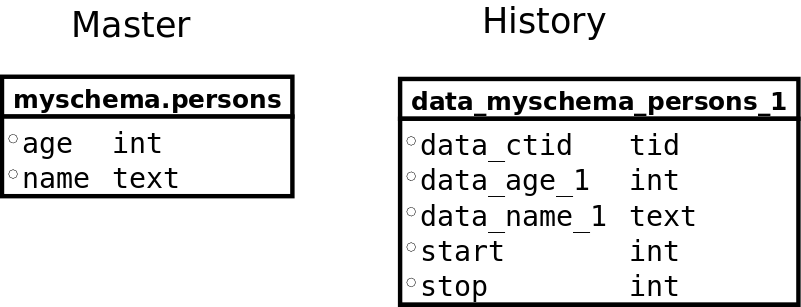
\includegraphics[width=0.5\textwidth]{history-data-table}
  \caption{An example of the schema of a data table in the history database}
  \label{history-data-table}
\end{figure}

\subsection{Populating and updating the history database}
When the history database is initialized its contents are not read directly from the master database.
Instead there is a dedicated instance of Postgres that replicates the master database that is used as a reference for the history.
This instance is called \textit{slave}.
The reason for using another instance to read the schema and data from the master is the format of the write-ahead log, or WAL.

The contents of the WAL are used to update the history database with the changes that are made to the master after the history has been initialized.
This approach was chosen because it makes it possible to read the changes that are made to the master database without inspecting it directy, e.g. with triggers.
That was considered important in the design process for Marty because any change on the master might introduce bugs and reduce its performance.
However, the WAL contains binary information and to be able to read it and use its contents it is necessary to have the database cluster files from the master as a reference.
Instead of implementing a complex algorithm to read the contents of the WAL it was decided to leverage on the recovery feature of Postgres that reads the WAL and applies it to the database cluster.
The slave is therefor started with a copy of the cluster files from the master database and it then replays the WAL into the cluster as it arrives from the master.
As it does so it logs all the operations that it replays and Marty uses this log to find and read the new version of the data from the slave.

The WAL debug log that logs all the operations is not enabled by default and the slave must therefor be compiled with special flags to enable it.
The replay must also be paused after each transaction that has been replayed to give Marty time to read the data from that transaction before the next one is applied.
To be able to do that it is necessary to patch Postgres and so the slave therefor runs on a specially patched version of Postgres.
More information about the slave can be found in chapter TODO.

\section{Advantages and Drawbacks}
The current architecture of Marty that is described in this chapter was chosen because of its simplicity and because it could be implemented in high level code (PL/pgSQL instead of C) which sped up prototyping and simplified the development of Marty.
However, it has a few drawbacks which make it unsuitable for a production ready version of Marty.
The main drawback is the lack of optimization for queries from the clones to the history database; when a user queries a table in a clone database it fetches the complete contents of that table from the history database even if the query should only return a small part of it to the user.
Another issue is the creation of indexes for the tables in the clones; the user can not create indexes for the tables in the clone like she would create them on the master database.
This is because the tables that the user expects to find in the clone database are actually views and it is not possible to create indexes for views in Postgres.

See chapter TODO for a discussion of the current status of Marty, the limitations of the current version and ideas for future works and improvements.

\chapter{Implementation}
Marty is written in Python and PL/pgSQL with a small patch to the Postgres source code written in C.
Python and PL/pgSQL are both high-level programming languages and ideal for rapid prototyping.
The source code cointains two scripts, \textit{clone.py} and \textit{history.py}, which are used to create and populate the clone databases and the history database, respectively.
The patch to Postgres is necessary for Marty to be able to read the changes from the write-ahead log (WAL) with the slave instance.

Marty is designed to work with Postgres 9.3.3.
The patch is written for this version and might not work with other versions, older or newer.

This chapter describes the implementation of Marty.
It explains which parts of Postgres Marty uses to create the history database and keep track of the changes that are made to the master database.
It starts by explaining how the slave instance is used and why it is patched.
It then continues with a description of the history database and its design and ends with a description of the clone databases and how they use the history database to imitate the master.

\section{The slave instance}

\begin{wrapfigure}{r}{0.4\textwidth}
  \vspace{-20pt}
  \begin{center}
    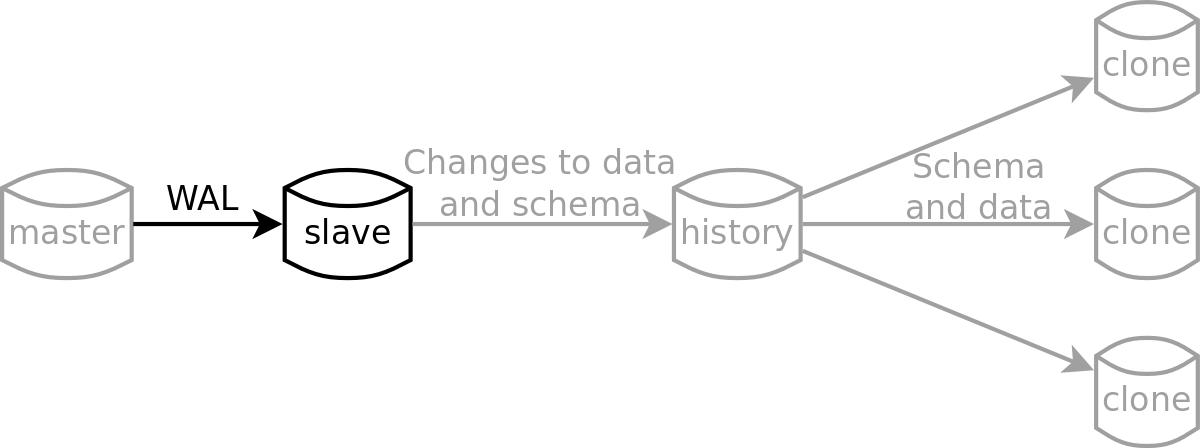
\includegraphics[width=0.38\textwidth]{img/architecture-slave}
  \end{center}
  \vspace{-20pt}
  \caption{The slave part of the architecture}
  \vspace{-10pt}
\end{wrapfigure}

Marty uses the slave instance to initialize the history database and to inspect the contents of the WAL from the master.
The slave is configured to act as a \textit{hot standby} for the master; it starts with a copy of the master database and updates it with the WAL from the master.
A hot standby can be queried with read only quries and when the slave database is first started Marty copies its schema and data to the history database.
It then inspects the changes from the WAL as they are applied and updates the history database accordingly.

Before the slave instance is started the database administrator that manages the master must configure it correctly.
This includes configuring a few parameters in the \textit{postgres.conf} file, see table \ref{table:master-config}.
Next the administrator must take a \textit{base-backup} of the master database.
This can be done with the program \textit{pg\_basebackup} and might require changes to the \textit{pg\_hba.conf} file, see the Postgres documentation for further reference. % TODO add referernce?

\begin{table}[h]
  \centering
  \texttt{
    \begin{tabular}{| l | l |}
      \hline
      \textbf{Parameter} & \textbf{Value} \\ \hline
      wal\_level & hot\_standby \\ \hline
      archive\_mode & on \\ \hline
      archive\_command & 'cp \%p /path/to/archive/\%f' \\ \hline
      max\_wal\_senders & 1 \\ \hline
    \end{tabular}
  }
  \caption{Configuration parameters in postgres.conf for the master database}
  \medskip
  \small
  This archive command is just an example, when the master is configured it must use an archive command that copies the WAL files to a storage where they are accessible by the slave.
  Also note that \texttt{max\_wal\_senders} must at least be 1, but can be higher.
  \label{table:master-config}
\end{table}

As previously noted the slave runs on a patched version of Postgres that must be compiled with a special flag that enables Postgres to log the WAL replay actions.
When the patch has been applied to the Postgres source code it must be compiled with the \texttt{WAL\_DEBUG} CPP flag.

Instead of creating a new cluster for the slave with the \texttt{initdb} command the administrator should use the files from the base-backup.
When they have been copied to the correct place the \textit{postgres.conf} file must be updated, see table \ref{table:slave-config}.
It is then necessary to add a \textit{recovery.conf} file with a command to fetch the WAL files from the master database, see the Postgres documentation for further reference. % TODO reference?

\begin{table}[h]
  \centering
  \texttt{
    \begin{tabular}{| l | l |}
      \hline
      \textbf{Parameter} & \textbf{Value} \\ \hline
      hot\_standby & on \\ \hline
      wal\_debug & on \\ \hline
    \end{tabular}
  }
  \caption{Configuration parameters in postgres.conf for the slave database}
  \label{table:slave-config}
\end{table}
\

\chapter{Benchmarks}
Maybe.

\chapter{Current status and future work}
\label{ch:current-status}
The current version of Marty is a proof of concept prototype.
It is written in Python and PL/pgSQL for version 9.3.3 of Postgres.
It supports replicating a database with ordinary tables without any default values or constraints.

Marty replicates a \textit{master} database and the replicas are called \textit{clone} databases.
They are standard Postgres databases that the user initializes with a Python script provided by Marty.
The tables in the clone databases are empty until they are queried.
This reduces the time it takes to create the clone database but with the drawback of a longer query time when the tables in the clones are first queried.
The lazy-loading of the tables is implemented with views.
When the user queries a table in a clone database like she would query it in the master database she is actually querying a view.
When a view is queried for the first time it calls a PL/pgSQL function that fetches the data and caches it on the clone database before it is returned.
Subsequent queries to the view use the cached data and thus they take less time.

The clone databases do not fetch the data directly from the master database.
In the time between initializing the clone with the empty tables and fetching their data when the user queries the tables in the database the state of the master database might have changed.
This could cause inconsistency in the clone database.
To prevent that it fetches the data from another database, the \textit{history} database.
It is a standard Postgres database that contains information about the schema and a copy of the data of the master database.
As the name suggests it contains a history of the changes that have been made on the master database, both to the schema and the data.
The clone can therefore query the history database for the data as it was at a certain point in time.
This guarantees the consistency of the data that the clone database fetches and returns to the user.

Marty uses the \textit{write-ahead log} (WAL) from the master database to monitor how it changes.
This log contains the changes of the master database in binary records that can be directly applied to the cluster files that store the contents of the database.
This makes it difficult or impossible to read the WAL without having a copy of the database cluster files as a reference.
Marty uses a dedicated instance of Postgres to read the contents of the WAL.
This is the \textit{slave} instance which is configured as a \textit{hot-standby} for the master database.
While it reads the WAL and replays it to the cluster files Marty inspects the changes that the WAL makes and records those changes in the history database.

\section{Limitations of the current version}
Marty can be used to quickly create databases for the development and testing of applications that use Postgres.
However, the current version is limited to a few core elements in a Postgres database.
Those are schemas, ordinary tables and the standard data types of the columns.
Marty does not replicate default values on columns or any column or table constraints, such as foreign keys or UNIQUE constraints.

Before Marty is ready for use in a production environment these limitations must be addressed.
Support must be added for default values and constraints, along with support for more types of database objects.
Marty should be able to replicate views as well as ordinary tables.
Primary keys in tables are often created with the \textit{serial} type which uses a \textit{sequence} to supply the table with values for the primary key.
Marty must be able to replicate sequences.

Ordinary tables, sequences and views are all examples of \textit{relations}.
Other relation types are \textit{TOAST tables}, \textit{materialized views}, \textit{composite types} and \textit{foreign tables}\footnote{http://www.postgresql.org/docs/9.3/static/catalog-pg-class.html}.
It would be nice to add support for these types of relations to make Marty usable in more enviroments.
Other types of database objects that could be supported in future versions are functions and operators, data types and domains, triggers and rewrite rules.

Another limitation of the current version is the design of the clone databases.
They use views to imitate tables that lazy-load their contents from another database.
This complicates some operations that a user might want to perform in the database, such as creating new indexes or altering the tables.
The user should be able to execute as many operations as possible in the clone databases in exactly the same way as they are executed in the master database.
This would likely require the user to run a patched version of Postgres for the clone databases.

The clone databases do not optimize their queries to the history database in any way.
When the user queries a table in the clone database it fetches the complete contents of that table from the history, even though the user limits the query results to only a few rows.
A patched version of Postgres could mitigate this and inspect the queries from the user before it fetches the data form the history database.
This could speed up the execution of queries, especially for tables that have many thousunds, or even millions of rows.

\section{Future work}
There are many features that can be added to Marty to make it more attractive to developers.
These include feature that minimize the overhead of using Marty, make it more secure or simplify its setup.
Below are a few ideas for improvements or additions that could be added to Marty in future versions.

\subsection{Logical replication}
\textit{Logical log streaming replication} is a feature that is being implemented for Postgres and will be part of future versions.
It provides the possibility of shipping the change log of one database instead of shipping the changes of the whole database cluster, like the write ahead log currently does.
The receiving database uses plugins to reads the contents of the logical log.
One plugin is used to apply the changes from the log but another one is available that creates SQL statements from the changes, without applying them.
Marty could provide one such plugin for the history database that would read the log and create new history versions.
This would make the slave instance in Marty unnecessary and would simplify its setup and maintenance.

\subsection{Data obfuscation}
Many databases contain sensitive information, or information that should not be used in a development or testing environment.
Examples of such data are credit card numbers and e-mail addresses.
Marty could include the possibility to change the values of certain columns in certain tables when it inserts data into the history database.
This could be in the form of a Python script which would allow for a very flexible way of obfuscating or changing the values before they are inserted into the history.
This would prevent the sensitive data from entering the development or testing environment, thus preventing any accidental use.

\subsection{VCS integration}
Version control systems (VCS) such as Git\footnote{http://git-scm.com} and Mercurial\footnote{http://mercurial.selenic.com} allow developers to work on many different features or fixes for a program simultaneously while keeping the changes for each feature isolated.
The developers create \textit{branches} of the source code where each branch contains the changes for only one feature or fix.
They can then switch between branches without polluting one branch with the changes from another one.

It is possible to create \textit{hooks} for these systems that run specific commands when the user executes certain actions.
Marty could include hooks that would automatically create and initialize a new clone database whenever a developer created a new branch.
They could also be configured to update the settings of the project that the developer is working on.
The developer would then always use the correct database for the active branch without needing to change manually from one database to another.
This could ease development as the developer would always get a new development database for each new branch.

\subsection{Time travel}
Time travel is a feature that was once a part of Postgres\footnote{http://www.postgresql.org/docs/6.3/static/c0503.htm}.
It allowed users to query the contents of the database as it was at a certain point in time in the past.
It was removed from Postgres in version 6.2 due to performance impact and how much extra storage was needed to support this feature.

It can, however, be useful in some situations to be able to query the database for historical versions of its data.
This is possible in the current version of Postgres by using the write-ahead log, but it is not a very practical solution.
The WAL must be applied to an old base-backup of the master database and Postgres must be configured to stop the WAL replay at the right moment.
This can be time consuming as the WAL replay can take considerable time.
It can also be hard to leap between different points in time when replaying the WAL as there is no way to rewind it.

The information in the history database can instead be used for this task.
It would be a relatively quick operation to jump backwards or forwards in time and inspect the different states of the database.
It is already possible to use Marty in such a way with minimal changes.
The user selects which version to inspect and creates a new clone database that is initialized for that version.
This includes some manual labor as the user must first find the correct history version and then configure Marty to initialize a clone database with that specific version ID.
It is also cumbersome to inspect different versions as the user would need to create a new clone database for each version and then query all of them and inspect the results manually.

Future versions of Marty could include a tool that would enable a user to quickly scan the history database and locate the correct history version.
The user could inspect the database as it was at that time and even compare two or more versions.
This would make it possible to debug anomalies that were caused by erronous data in the master database even after the database state has been altered and the anomalies have stopped.

\chapter{Conclusion}
Fin


\appendix
\renewcommand{\chaptername}{Appendix}

\chapter{Source code}
This is the source code for Marty.
It is accessible online at Github\footnote{https://github.com/baldurthoremilsson/marty/commit/f9a88d7}.

\definecolor{deepblue}{rgb}{0,0,0.5}
\definecolor{deepgreen}{rgb}{0,0.5,0}

\lstset{
  basicstyle=\tiny\ttfamily,
  breaklines=true,
  captionpos=t,
  language=Python,
  numbers=left,
  xleftmargin=2em,
  keywordstyle=\bfseries\color{deepblue},
  stringstyle=\color{deepgreen},
}

\begin{lstlisting}[caption={clone.py}]
#!/usr/bin/env python
# -*- coding: utf-8 -*-

import sys
import argparse
import psycopg2
from utils import HistoryInspector, ClonePopulator, get_logger


def connect(history, clone):
    histcon = psycopg2.connect(**history)
    clonecon = psycopg2.connect(**clone)
    histcon.autocommit = True
    clonecon.autocommit = True
    return histcon, clonecon


def main():
    parser = argparse.ArgumentParser()
    parser.add_argument('--history-host', help='Hostname or IP of the history database')
    parser.add_argument('--history-port', help='Port number for the history database')
    parser.add_argument('--history-user', help='Username for the history database')
    parser.add_argument('--history-password', help='Password for the history database')
    parser.add_argument('--history-database', help='Name of the history database')

    parser.add_argument('--clone-host', help='Hostname or IP of the clone database')
    parser.add_argument('--clone-port', help='Port number for the clone database')
    parser.add_argument('--clone-user', help='Username for the clone database')
    parser.add_argument('--clone-password', help='Password for the clone database')
    parser.add_argument('--clone-database', help='Name of the clone database')

    args = parser.parse_args()

    history = {
        'host': args.history_host,
        'port': args.history_port,
        'user': args.history_user,
        'password': args.history_password,
        'database': args.history_database
    }

    clone = {
        'host': args.clone_host,
        'port': args.clone_port,
        'user': args.clone_user,
        'password': args.clone_password,
        'database': args.clone_database
    }

    histcon, clonecon = connect(history, clone)

    inspector_logger = get_logger('inspector')
    populator_logger = get_logger('populator')

    inspector = HistoryInspector(histcon, logger=inspector_logger)
    populator = ClonePopulator(clonecon, inspector.update, history, logger=populator_logger)
    populator.initialize()
    for schema in inspector.schemas():
        populator.create_schema(schema)
        for table in inspector.tables(schema):
            inspector.columns(table)
            populator.create_table(table)
    clonecon.commit()


if __name__ == '__main__':
    main()
\end{lstlisting}
\begin{lstlisting}[caption={history.py}]
#!/usr/bin/env python
# -*- coding: utf-8 -*-

import psycopg2
import sys
import argparse
import re

from utils import SlaveInspector, HistoryPopulator, get_logger
from utils.dbobjects import Schema


class RegExer(object):
    def __init__(self):
        self.m = None

        rel_tid = 'rel (?P<spc_node>\d+)/(?P<db_node>\d+)/(?P<rel_node>\d+); tid (?P<block>\d+)/(?P<offset>\d+)'

        self.regexes = {
            'insert': re.compile(r'Heap - insert(?:\(init\))?: {}'.format(rel_tid)),
            'update': re.compile(r'Heap - (?:hot_)?update: {} xmax \d+ (?:[A-Z_]+ )?; new tid (?P<new_block>\d+)/(?P<new_offset>\d+) xmax \d+'.format(rel_tid)),
            'delete': re.compile(r'Heap - delete: {}'.format(rel_tid)),
            'lastup': re.compile(r'LOG:  database system was interrupted; last known up at (?P<timestamp>\d{4}-\d{2}-\d{2} \d{2}:\d{2}:\d{2})'),
            'connect': re.compile(r'LOG:  database system is ready to accept read only connections'),
            'paused': re.compile(r'LOG:  recovery has paused'),
            'redo': re.compile(r'LOG:  REDO @ [0-9A-F]+/[0-9A-F]+; LSN [0-9A-F]+/[0-9A-F]+: prev [0-9A-F]+/[0-9A-F]+; xid [0-9]+; len [0-9]+(?:; bkpb[0-9]+)?: (.*)'),
            'commit': re.compile(r'Transaction - commit: (?P<timestamp>\d{4}-\d{2}-\d{2} \d{2}:\d{2}:\d{2}\.\d+)'),
        }

    def match(self, regex, pattern):
        self.m = self.regexes[regex].match(pattern)
        return self.m

    @property
    def groupdict(self):
        return self.m.groupdict()

    def __getitem__(self, key):
        return self.groupdict[key]

    def get(self, key, val):
        try:
            return self[key]
        except KeyError:
            return val



class Worker(object):
    def __init__(self, infile, regexer, connect_callback):
        self.infile = infile
        self.regexer = regexer
        self.connect_callback = connect_callback
        self.inspector = None
        self.populator = None
        self.slavecon = None
        self._work = []
        self._commited = False
        self._timestamp = None

    def consume(self):
        self.infile.flush()
        line = self.infile.readline()
        if self.regexer.match('lastup', line):
            self._timestamp = self.regexer.m.groupdict()['timestamp']
        elif self.regexer.match('connect', line):
            self.slavecon, self.inspector, self.populator = self.connect_callback(self._timestamp)
            self.inspector.resume()
            self._timestamp = None
        elif self.regexer.match('paused', line):
            if self.inspector:
                self.inspector.resume()
        elif self.regexer.match('redo', line):
            work = self.regexer.m.groups()[0]
            if self.regexer.match('commit', work):
                if self.inspector:
                    self._commited = True
                    self._timestamp = self.regexer.m.groupdict()['timestamp']
            elif self._commited:
                self.populator.update(self._timestamp)
                for w in self._work:
                    self.work(w)
                self._work = []
                self._commited = False
                self._timestamp = None
            self._work.append(work)

    def work(self, work):
        for action in 'insert', 'update', 'delete':
            if self.regexer.match(action, work):
                break
        else:
            # If the work is not an insert, update or delete action we leave
            # (we only run the else part if the for loop does not break)
            return

        db_node = int(self.regexer.get('db_node', 0))
        rel_node = int(self.regexer.get('rel_node', 0))
        block = int(self.regexer.get('block', 0))
        offset = int(self.regexer.get('offset', 0))
        new_block = int(self.regexer.get('new_block', 0))
        new_offset = int(self.regexer.get('new_offset', 0))

        if db_node != self.inspector.db_oid:
            return

        if rel_node in self.inspector.system_tables:
            table = self.inspector.system_tables[rel_node]
            if table.name == 'pg_namespace':
                self.schema_change(action, block, offset, new_block, new_offset)
            elif table.name == 'pg_class':
                self.table_change(action, block, offset, new_block, new_offset)
            elif table.name == 'pg_attribute':
                self.column_change(action, block, offset, new_block, new_offset)
            return

        table = self.inspector.tabledict.get(rel_node, None)
        if not table:
            return

        if action == 'insert':
            self.insert(table, block, offset)
        elif action == 'update':
            self.update(table, block, offset, new_block, new_offset)
        elif action == 'delete':
            self.delete(table, block, offset)

    def ctid(self, block, offset):
        return '({},{})'.format(block, offset)

    def schema_change(self, action, block, offset, new_block, new_offset):
        if action == 'insert':
            schema = self.inspector.get_schema(self.ctid(block, offset))
            self.populator.add_schema(schema)
        elif action == 'update':
            schema = self.inspector.get_schema(self.ctid(new_block, new_offset))
            self.populator.add_schema(schema)
            self.populator.remove_schema(self.ctid(block, offset))
        elif action == 'delete':
            self.populator.remove_schema(self.ctid(block, offset))

    def table_change(self, action, block, offset, new_block, new_offset):
        if action == 'insert':
            table = self.inspector.get_table(self.ctid(block, offset))
            if table:
                self.populator.add_table(table)
                self.populator.create_table(table)
        elif action == 'update':
            table = self.inspector.get_table(self.ctid(new_block, new_offset))
            if table:
                self.populator.add_table(table)
            self.populator.remove_table(self.ctid(block, offset))
        elif action == 'delete':
            table = self.populator.get_table(self.ctid(block, offset))
            if table:
                self.populator.delete_all(table)
            self.populator.remove_table(self.ctid(block, offset))

    def column_change(self, action, block, offset, new_block, new_offset):
        update = self.populator.update_id
        if action == 'insert':
            column = self.inspector.get_column(self.ctid(block, offset), update=update)
            if column:
                self.populator.add_column(column)
                self.populator.add_data_column(column)
        if action == 'update':
            old_column = self.populator.get_column(self.ctid(block, offset))
            column = self.inspector.get_column(self.ctid(new_block, new_offset),
                    update=update, internal_name=old_column.internal_name)
            if column:
                self.populator.add_column(column)
            self.populator.remove_column(self.ctid(block, offset))
        if action == 'delete':
            self.populator.remove_column(self.ctid(block, offset))

    def insert(self, table, block, offset):
        row = self.inspector.get(table, block, offset)
        self.populator.insert(table, block, offset, row)

    def update(self, table, block, offset, new_block, new_offset):
        self.delete(table, block, offset)
        self.insert(table, new_block, new_offset)

    def delete(self, table, block, offset):
        self.populator.delete(table, block, offset)


def connect(slave, history):
    slavecon = psycopg2.connect(**slave)
    histcon = psycopg2.connect(**history)
    slavecon.autocommit = True
    histcon.autocommit = True
    return slavecon, histcon

def connect_callback(timestamp):
    parser = argparse.ArgumentParser()

    parser.add_argument('--slave-host', help='Hostname or IP of the slave database')
    parser.add_argument('--slave-port', help='Port number for the slave database')
    parser.add_argument('--slave-user', help='Username for the slave database')
    parser.add_argument('--slave-password', help='Password for the slave database')
    parser.add_argument('--slave-database', help='Name of the slave database')

    parser.add_argument('--history-host', help='Hostname or IP of the history database')
    parser.add_argument('--history-port', help='Port number for the history database')
    parser.add_argument('--history-user', help='Username for the history database')
    parser.add_argument('--history-password', help='Password for the history database')
    parser.add_argument('--history-database', help='Name of the history database')

    args = parser.parse_args()

    slave = {
        'host': args.slave_host,
        'port': args.slave_port,
        'user': args.slave_user,
        'password': args.slave_password,
        'database': args.slave_database
    }

    history = {
        'host': args.history_host,
        'port': args.history_port,
        'user': args.history_user,
        'password': args.history_password,
        'database': args.history_database
    }


    slavecon, histcon = connect(slave, history)

    inspector_logger = get_logger('inspector')
    populator_logger = get_logger('populator')

    inspector = SlaveInspector(slavecon, logger=inspector_logger)
    populator = HistoryPopulator(histcon, logger=populator_logger)

    populator.create_tables()
    populator.update(timestamp)
    for schema in inspector.schemas():
        populator.add_schema(schema)
        for table in inspector.tables(schema):
            inspector.columns(table)
            populator.add_table(table)
            populator.create_table(table)
            populator.fill_table(table)

    return slavecon, inspector, populator


def main():
    worker = Worker(sys.stdin, RegExer(), connect_callback)
    while True:
        worker.consume()


if __name__ == "__main__":
    main()
\end{lstlisting}
\begin{lstlisting}[caption={utils/\_\_init\_\_.py}]
# -*- coding: utf-8 -*-

import sys
import logging

from inspector import SlaveInspector, HistoryInspector
from populator import HistoryPopulator, ClonePopulator


__all__ = ('SlaveInspector', 'HistoryInspector', 'HistoryPopulator',
        'ClonePopulator', 'get_logger')


def get_logger(name):
    formatter = logging.Formatter(logging.BASIC_FORMAT)
    handler = logging.StreamHandler(sys.stdout)
    handler.setFormatter(formatter)
    logger = logging.getLogger(name)
    logger.addHandler(handler)
    logger.setLevel(logging.DEBUG)
    return logger
\end{lstlisting}
\begin{lstlisting}[caption={utils/dbobjects.py}]
# -*- coding: utf-8 -*-

class Schema(object):

    def __init__(self, ctid, oid, name):
        self.ctid = ctid
        self.oid = oid
        self.name = name

    def __repr__(self):
        return u'<Schema {} ({})>'.format(self.name, self.oid)


class Table(object):

    def __init__(self, schema, ctid, oid, name, con=None, internal_name=None):
        self.schema = schema
        self.ctid = ctid
        self.oid = oid
        self.name = name
        self.columns = []
        self.con = con
        self._internal_name = internal_name
        self.update = None

    def __repr__(self):
        return u'<Table {} ({})>'.format(self.name, self.oid)

    @property
    def long_name(self):
        return '{}.{}'.format(self.schema.name, self.name)

    @property
    def internal_name(self):
        if not self._internal_name:
            self._internal_name = 'data_{}_{}_{}'.format(self.schema.name, self.name, self.update)
        return self._internal_name

    @property
    def internal_columns(self):
        yield CTIDColumn()
        for column in self.columns:
            yield column
        yield StartColumn()
        yield StopColumn()

    def add_column(self, ctid, name, number, type, length, internal_name=None):
        self.columns.append(Column(self, ctid, name, number, type, length, internal_name=internal_name))

    def data(self):
        with self.con.cursor() as curs:
            curs.execute('SELECT ctid, * FROM {}'.format(self.long_name))
            for row in curs:
                yield row


class Column(object):

    def __init__(self, table, ctid, name, number, type, length, internal_name=None):
        self.ctid = ctid
        self.table = table
        self.name = name
        self.number = number
        self.type = type
        self.length = length
        self._internal_name = internal_name

    def __repr__(self):
        return u'<Column {} {}({})>'.format(self.name, self.type, self.length)

    @property
    def internal_name(self):
        if not self._internal_name:
            self._internal_name = 'data_{}_{}'.format(self.name, self.table.update)
        return self._internal_name


class CTIDColumn(object):
    internal_name = 'data_ctid'
    type = 'tid'
    length = -1


class StartColumn(object):
    internal_name = 'start'
    type = 'integer REFERENCES marty_updates(id) NOT NULL'
    length = -1


class StopColumn(object):
    internal_name = 'stop'
    type = 'integer REFERENCES marty_updates(id)'
    length = -1
\end{lstlisting}
\begin{lstlisting}[caption={utils/inspector.py}]
# -*- coding: utf-8 -*-

from dbobjects import Schema, Table, Column, StartColumn, StopColumn

class SlaveInspector(object):

    def __init__(self, con, logger=None):
        self.con = con
        self.db_oid = self._get_db_oid()
        self.tabledict = {}
        self._system_tables = None
        self.pg_namespace = None
        if logger:
            self.logger = logger
        else:
            self.logger = logging.getLogger()
            self.logger.addHandler(logging.NullHandler())

    def _get_db_oid(self):
        with self.con.cursor() as curs:
            curs.execute('SELECT oid FROM pg_database WHERE datname = current_database()')
            row = curs.fetchone()
            return row[0]

    def schemas(self):
        with self.con.cursor() as curs:
            curs.execute("""
            SELECT ctid, oid, nspname
            FROM pg_namespace
            WHERE nspname NOT LIKE 'information_schema' AND nspname NOT LIKE 'pg_%'
            """)
            for ctid, oid, name in curs:
                self.logger.info('schema {}, {}, {}'.format(ctid, oid, name))
                yield Schema(ctid, oid, name)

    def tables(self, schema):
        """
        Missing:
            indexes (relkind = i)
            sequences (relkind = S)
            views (relkind = v)
            materialized views (relkind = m)
            composite type (relkind = c)
            TOAST tables (relkind = t)
            foreign tables (relkind = f)
        """
        with self.con.cursor() as curs:
            curs.execute("""
            SELECT ctid, oid, relname, pg_catalog.pg_relation_filenode(oid) AS filenode
            FROM pg_class
            WHERE relnamespace = %s AND relkind = 'r'
            """, (schema.oid,))
            for ctid, oid, name, filenode in curs:
                self.logger.info('table {}, {} ({})'.format(oid, name, filenode))
                table = Table(schema, ctid, oid, name, con=self.con)
                self.tabledict[filenode] = table
                yield table

    def columns(self, table):
        """
        Missing:
            arrays (attndims)
            data in TOAST tables (attstorage)
            not null (attnotnull)
            default value (atthasdef)
            attislocal?
            attinhcount?
            collation (attcollation)
            attoptions?
            attfdwoptions?
        """
        with self.con.cursor() as curs:
            curs.execute("""
            SELECT pg_attribute.ctid, attname, attnum, typname, atttypmod
            FROM pg_attribute
            LEFT JOIN pg_type ON pg_attribute.atttypid = pg_type.oid
            WHERE attrelid = %s AND attisdropped = false AND attnum > 0
            ORDER BY attnum ASC
            """, (table.oid,))
            for ctid, name, number, type, length in curs:
                self.logger.info('column {} {}({})'.format(name, type, length))
                table.add_column(ctid, name, number, type, length)

    @property
    def system_tables(self):
        """
        This looks up tables
            pg_namespace
            pg_class
        """
        if self._system_tables == None:
            self._system_tables = {}
            schema = Schema(None, None, 'pg_catalog')
            with self.con.cursor() as curs:
                curs.execute("""
                SELECT ctid, oid, relname, pg_catalog.pg_relation_filenode(oid) as filenode
                FROM pg_class
                WHERE relname IN ('pg_namespace', 'pg_class', 'pg_attribute')
                """)
                for ctid, oid, name, filenode in curs:
                    self.logger.info('system table {}, {} ({})'.format(oid, name, filenode))
                    table = Table(schema, ctid, oid, name, con=self.con)
                    self._system_tables[filenode] = table
        return self._system_tables

    def get_schema(self, ctid=None, oid=None):
        query = 'SELECT ctid, oid, nspname FROM pg_namespace '
        if oid:
            query += 'WHERE oid = %s'
            values = (oid,)
        else:
            query += 'WHERE ctid = %s'
            values = (ctid,)
        with self.con.cursor() as curs:
            curs.execute(query, values)
            ctid, oid, nspname = curs.fetchone()
            return Schema(ctid, oid, nspname)

    def get_table(self, ctid=None, oid=None):
        query = 'SELECT ctid, oid, relname, relnamespace, relkind FROM pg_class WHERE relkind = %s AND '
        values = ['r']
        if oid:
            query += 'oid = %s'
            values.append(oid)
        else:
            query += 'ctid = %s'
            values.append(ctid)
        with self.con.cursor() as curs:
            curs.execute(query, values)
            ctid, oid, relname, relnamespace, relkind = curs.fetchone()
            schema = self.get_schema(oid=relnamespace)
            return Table(schema, ctid, oid, relname)

    def get_column(self, ctid=None, oid=None, update=None, internal_name=None):
        query = """
        SELECT pg_attribute.ctid, attrelid, attname, attnum, typname, atttypmod
        FROM pg_attribute
        LEFT JOIN pg_type ON pg_attribute.atttypid = pg_type.oid
        WHERE %s AND attisdropped = false AND attnum > 0
        ORDER BY attnum ASC
        """
        if oid:
            query %= 'attrelid = %s'
            values = (oid,)
        else:
            query %= 'pg_attribute.ctid = %s'
            values = (ctid,)
        with self.con.cursor() as curs:
            curs.execute(query, values)
            row = curs.fetchone()
            if not row:
                return None
            ctid, attrelid, attname, attnum, typname, atttypmod = row
            table = self.get_table(oid=attrelid)
            table.update = update
            return Column(table, ctid, attname, attnum, typname, atttypmod, internal_name=internal_name)

    def resume(self):
        self.logger.info('resuming')
        with self.con.cursor() as curs:
            curs.execute('SELECT pg_xlog_replay_resume()')

    def get(self, table, block, offset, cols=None):
        with self.con.cursor() as curs:
            if cols:
                cols = ', '.join(cols)
            else:
                cols = '*'
            query = "SELECT {} FROM {} WHERE ctid = '({},{})'"
            query = query.format(cols, table.long_name, block, offset)
            curs.execute(query)
            row = curs.fetchone()
            return row


class HistoryInspector(object):

    def __init__(self, con, logger=None):
        self.con = con
        if logger:
            self.logger = logger
        else:
            self.logger = logging.getLogger()
            self.logger.addHandler(logging.NullHandler())
        self.update = self._update()

    def _update(self):
        with self.con.cursor() as curs:
            curs.execute("""
            SELECT id, time
            FROM marty_updates
            ORDER BY time DESC LIMIT 1
            """)
            update_id, time = curs.fetchone()
            self.logger.debug('got update id {} from {}'.format(update_id, time))
            return update_id

    def schemas(self):
        with self.con.cursor() as curs:
            curs.execute("""
            SELECT _ctid, oid, name
            FROM marty_schemas
            WHERE start <= %(update_id)s AND (stop IS NULL OR stop > %(update_id)s)
            """, {'update_id': self.update})
            for ctid, oid, name, in curs:
                yield Schema(ctid, oid, name)

    def tables(self, schema):
        with self.con.cursor() as curs:
            curs.execute("""
            SELECT oid, ctid, name, internal_name
            FROM marty_tables
            WHERE schema = %(schema_id)s
              AND start <= %(update_id)s AND (stop IS NULL OR stop > %(update_id)s)
            """, {'schema_id': schema.oid, 'update_id': self.update})
            for oid, ctid, name, internal_name in curs:
                yield Table(schema, ctid, oid, name, internal_name=internal_name)

    def columns(self, table):
        with self.con.cursor() as curs:
            curs.execute("""
            SELECT ctid, name, number, type, length, internal_name
            FROM marty_columns
            WHERE table_oid = %(table_oid)s
              AND start <= %(update_id)s AND (stop IS NULL OR stop > %(update_id)s)
            ORDER BY number ASC
            """, {'table_oid': table.oid, 'update_id': self.update})
            for ctid, name, number, type, length, internal_name in curs:
                table.add_column(ctid, name, number, type, length, internal_name=internal_name)
\end{lstlisting}
\begin{lstlisting}[caption={utils/populator.py}]
# -*- coding: utf-8 -*-

import logging

from dbobjects import Table, Column


class HistoryPopulator(object):

    def __init__(self, con, logger=None):
        self.con = con
        self.update_id = None
        if logger:
            self.logger = logger
        else:
            self.logger = logging.getLogger()
            self.logger.addHandler(logging.NullHandler())

    def create_tables(self):
        self.logger.info('creating tables')

        with self.con.cursor() as curs:
            # marty_updates
            curs.execute("""
            CREATE TABLE IF NOT EXISTS marty_updates(
                id SERIAL PRIMARY KEY,
                time TIMESTAMP DEFAULT current_timestamp NOT NULL,
                mastertime TIMESTAMP NOT NULL
            )
            """)

            # marty_schemas
            curs.execute("""
            CREATE TABLE IF NOT EXISTS marty_schemas(
                _ctid tid NOT NULL,
                oid oid NOT NULL,
                name name NOT NULL,
                start integer REFERENCES marty_updates(id) NOT NULL,
                stop integer REFERENCES marty_updates(id)
            )
            """)

            # marty_tables
            curs.execute("""
            CREATE TABLE IF NOT EXISTS marty_tables(
                _ctid tid NOT NULL,
                oid oid NOT NULL,
                name name NOT NULL,
                schema oid NOT NULL,
                internal_name name NOT NULL,
                start integer REFERENCES marty_updates(id) NOT NULL,
                stop integer REFERENCES marty_updates(id)
            )
            """)

            # marty_columns
            curs.execute("""
            CREATE TABLE IF NOT EXISTS marty_columns(
                _ctid tid NOT NULL,
                table_oid oid NOT NULL,
                name name NOT NULL,
                number int2 NOT NULL,
                type name NOT NULL,
                length int4 NOT NULL,
                internal_name name NOT NULL,
                start integer REFERENCES marty_updates(id) NOT NULL,
                stop integer REFERENCES marty_updates(id)
            )
            """)

    def update(self, mastertime):
        with self.con.cursor() as curs:
            curs.execute("""
            INSERT INTO marty_updates(mastertime) VALUES(%s) RETURNING id
            """, (mastertime,))
            self.update_id = curs.fetchone()[0]
            self.logger.debug('new update id {}'.format(self.update_id))

    def add_schema(self, schema):
        self.logger.info('adding schema {}'.format(schema.name))

        with self.con.cursor() as curs:
            curs.execute("""
            INSERT INTO marty_schemas(_ctid, oid, name, start) VALUES(%s, %s, %s, %s)
            """, (schema.ctid, schema.oid, schema.name, self.update_id))

    def remove_schema(self, ctid):
        self.logger.info('removing schema {}'.format(ctid))

        with self.con.cursor() as curs:
            curs.execute("""
            UPDATE marty_schemas SET stop = %s WHERE _ctid = %s
            """, (self.update_id, ctid))

    def add_table(self, table):
        self.logger.info('adding table {}'.format(table.long_name))

        update = self.update_id
        table.update = update
        with self.con.cursor() as curs:
            curs.execute("""
            INSERT INTO marty_tables(_ctid, oid, name, schema, internal_name, start)
            VALUES(%s, %s, %s, %s, %s, %s)
            """, (table.ctid, table.oid, table.name, table.schema.oid, table.internal_name, self.update_id))

            self.logger.debug(curs.query)

            for column in table.columns:
                self.add_column(column)

    def remove_table(self, ctid):
        self.logger.info('removing table {}'.format(ctid))

        with self.con.cursor() as curs:
            curs.execute("""
            UPDATE marty_tables SET stop = %s WHERE _ctid = %s
            """, (self.update_id, ctid))

    def add_column(self, column):
        self.logger.info('adding column {} to {}'.format(column.name, column.table.long_name))

        with self.con.cursor() as curs:
            curs.execute("""
            INSERT INTO marty_columns(_ctid, table_oid, name, number, type, length, internal_name, start)
            VALUES(%s, %s, %s, %s, %s, %s, %s, %s)
            """, (column.ctid, column.table.oid, column.name, column.number, column.type,
                column.length, column.internal_name, self.update_id))

            self.logger.debug(curs.query)

    def remove_column(self, ctid):
        self.logger.info('removing column {}'.format(ctid))

        with self.con.cursor() as curs:
            curs.execute("""
            UPDATE marty_columns SET stop = %s WHERE _ctid = %s
            """, (self.update_id, ctid))

    def create_table(self, table):
        self.logger.info('creating table {}'.format(table.internal_name))

        with self.con.cursor() as curs:
            cols = ','.join('\n  {} {}'.format(column.internal_name, column.type) for column in table.internal_columns)
            curs.execute('CREATE TABLE {}({})'.format(table.internal_name, cols))

            self.logger.debug(curs.query)

            curs.execute('SELECT oid FROM pg_class WHERE relname = %s', (table.internal_name,))
            table_oid, = curs.fetchone()

            for column in table.columns:
                curs.execute("""
                UPDATE pg_attribute
                SET atttypmod = %s
                WHERE attrelid = %s AND attname = %s
                """, (column.length, table_oid, column.internal_name))

    def add_data_column(self, column):
        with self.con.cursor() as curs:
            curs.execute("""
            ALTER TABLE {} ADD COLUMN {} {}
            """.format(column.table.internal_name, column.internal_name, column.type))

            curs.execute('SELECT oid FROM pg_class WHERE relname = %s', (column.table.internal_name,))
            table_oid, = curs.fetchone()

            curs.execute("""
            UPDATE pg_attribute
            SET atttypmod = %s
            WHERE attrelid = %s AND attname = %s
            """, (column.length, table_oid, column.internal_name))

    def fill_table(self, table):
        self.logger.info('filling table {}'.format(table.internal_name))

        table_name = table.internal_name
        column_names = ', '.join(column.internal_name for column in table.internal_columns)
        value_list = ', '.join('%s' for column in table.internal_columns)
        query = 'INSERT INTO {}({}) VALUES({})'.format(table_name, column_names, value_list)

        with self.con.cursor() as curs:
            for line in table.data():
                values = list(line)
                values.extend([self.update_id, None])
                curs.execute(query, values)

                self.logger.debug(curs.query)

    def insert(self, table, block, offset, row):
        self.logger.info('inserting to table {}'.format(table.internal_name))
        table_name = table.internal_name
        column_names = ', '.join(column.internal_name for column in table.internal_columns)
        value_list = ', '.join('%s' for column in table.internal_columns)
        query = 'INSERT INTO {}({}) VALUES({})'.format(table_name, column_names, value_list)

        values = ['({},{})'.format(block, offset)] + list(row) + [self.update_id, None]
        with self.con.cursor() as curs:
            curs.execute(query, values)
            self.logger.debug(curs.query)

    def delete(self, table, block, offset):
        self.logger.info('deleting from table {}'.format(table.internal_name))
        query = 'UPDATE {} SET stop = %s WHERE data_ctid = %s'.format(table.internal_name)
        values = [self.update_id, '({},{})'.format(block, offset)]
        with self.con.cursor() as curs:
            curs.execute(query, values)
            self.logger.debug(curs.query)

    def delete_all(self, table):
        query = 'UPDATE {} SET stop = %s WHERE stop IS NULL'.format(table.internal_name)
        values = (self.update_id,)
        with self.con.cursor() as curs:
            curs.execute(query, values)

    def get_table(self, ctid):
        with self.con.cursor() as curs:
            curs.execute("""
            SELECT _ctid, oid, name, internal_name
            FROM marty_tables
            WHERE _ctid = %s""", (ctid,))
            row = curs.fetchone()
            if not row:
                return
            ctid, oid, name, internal_name = row
            return Table(None, ctid, oid, name, internal_name=internal_name)

    def get_column(self, ctid):
        with self.con.cursor() as curs:
            curs.execute("""
            SELECT _ctid, table_oid, name, number, type, length, internal_name
            FROM marty_columns
            WHERE _ctid = %s""", (ctid,))
            row = curs.fetchone()
            if not row:
                return
            ctid, table_oid, name, number, type, length, internal_name = row
            return Column(None, ctid, name, number, type, length, internal_name=internal_name)


class ClonePopulator(object):

    def __init__(self, con, update, history_coninfo, logger=None):
        self.con = con
        self.update = update
        self.history_coninfo = history_coninfo
        if logger:
            self.logger = logger
        else:
            self.logger = logging.getLogger()
            self.logger.addHandler(logging.NullHandler())

    def initialize(self):
        with self.con.cursor() as curs:
            curs.execute('CREATE SCHEMA IF NOT EXISTS marty')
            curs.execute('CREATE EXTENSION IF NOT EXISTS dblink')
            curs.execute("""
            CREATE TABLE marty.bookkeeping(
                view_name name UNIQUE,
                local_table name,
                cached boolean DEFAULT false,
                coldef text,
                remote_select_stmt text,
                temp_table_def text
            )
            """)

            curs.execute("""
            CREATE FUNCTION coninfo() RETURNS text AS $$
            BEGIN
                RETURN '{coninfo}';
            END;
            $$ LANGUAGE plpgsql;
            """.format(coninfo=self._dblink_connstr()))

            curs.execute("""
            CREATE FUNCTION view_select(my_view_name text) RETURNS SETOF RECORD AS $$
            DECLARE
                view_info RECORD;
            BEGIN
                SELECT * FROM marty.bookkeeping WHERE view_name = my_view_name INTO view_info;
                IF NOT view_info.cached THEN
                    RAISE NOTICE 'fetching %', view_info.view_name;
                    EXECUTE ' INSERT INTO ' || view_info.local_table ||
                            ' SELECT ' || view_info.coldef ||
                            ' FROM dblink(''' || coninfo() || ''', ''' || view_info.remote_select_stmt || ''')'
                            ' AS ' || view_info.temp_table_def;
                    UPDATE marty.bookkeeping SET cached = true WHERE view_name = my_view_name;
                END IF;
                RETURN QUERY EXECUTE 'SELECT ' || view_info.coldef || ' FROM ' || view_info.local_table;
            END;
            $$ LANGUAGE plpgsql;
            """)

    def _dblink_connstr(self):
        parts = {
            'host': 'host={}',
            'port': 'port={}',
            'user': 'user={}',
            'password': 'password={}',
            'database': 'dbname={}',
        }
        return ' '.join(parts[key].format(value) for key, value in self.history_coninfo.iteritems())

    def create_schema(self, schema):
        self.logger.info('Creating schema {}'.format(schema.name))
        with self.con.cursor() as curs:
            curs.execute('CREATE SCHEMA IF NOT EXISTS {}'.format(schema.name))

    def create_table(self, table):
        self.logger.info('Creating table {}'.format(table.long_name))

        # Create table for local data
        table.update = self.update
        query = 'CREATE TABLE marty.{table}({cols})'
        cols = ','.join('\n  "{name}" {type}'.format(name=column.name, type=column.type) for column in table.columns)
        with self.con.cursor() as curs:
            curs.execute(query.format(table=table.internal_name, cols=cols))
            for column in table.columns:
                curs.execute("""
                UPDATE pg_attribute
                SET atttypmod = %(column_length)s
                WHERE attrelid = %(table_name)s::regclass::oid AND attname = %(column_name)s
                """, {'column_length': column.length, 'table_name': 'marty.{}'.format(table.internal_name), 'column_name': column.name})


            # Create view that combines local and remote data
            my_cols = ', '.join(['"{}"'.format(col.name) for col in table.columns])
            temp_columns = ['"{name}" {type}'.format(name=col.name, type=col.type) for col in table.columns]
            temp_table_def = 't1({columns})'.format(columns=', '.join(temp_columns))

            view_query = """
            CREATE VIEW {view_name}
            AS SELECT {cols} FROM view_select('{view_name}')
            AS {tabledef};
            """
            curs.execute(view_query.format(view_name=table.long_name, cols=my_cols, tabledef=temp_table_def))

            bookkeeping_query = """
            INSERT INTO marty.bookkeeping(view_name, local_table, coldef, remote_select_stmt, temp_table_def)
            VALUES(%(view_name)s, %(local_table)s, %(coldef)s, %(remote_select_stmt)s, %(temp_table_def)s);
            """
            local_cols = ', '.join(['"{}"'.format(col.name) for col in table.columns])
            internal_cols = ', '.join([col.internal_name for col in table.columns])
            remote_select_stmt = 'SELECT {cols} FROM {table} WHERE start <= {update} and (stop IS NULL or stop > {update})'
            bookkeeping_values = {
                'view_name': table.long_name,
                'local_table': 'marty.' + table.internal_name,
                'coldef': local_cols,
                'remote_select_stmt': remote_select_stmt.format(cols=internal_cols, table=table.internal_name, update=self.update),
                'temp_table_def': temp_table_def,
            }
            curs.execute(bookkeeping_query, bookkeeping_values)

            trigger_queries_values = {
                'trigger_name': table.long_name.replace('.', '_'),
                'local_table': 'marty.' + table.internal_name,
                'local_columns': my_cols,
                'new_values_insert': ', '.join(['NEW.' + col.name for col in table.columns]),
                'new_values_update': ', '.join(['"{name}" = NEW.{name}'.format(name=col.name) for col in table.columns]),
                'old_values': ' AND '.join(['"{name}" = OLD.{name}'.format(name=col.name) for col in table.columns]),
                'view_name': table.long_name,
            }

            # Create insert trigger for view
            insert_query = """
            CREATE FUNCTION {trigger_name}_insert() RETURNS trigger AS $$
                BEGIN
                    INSERT INTO {local_table}({local_columns}) VALUES({new_values_insert});
                    RETURN NEW;
                END;
            $$ LANGUAGE plpgsql;

            CREATE TRIGGER {trigger_name}_insert_trigger
            INSTEAD OF INSERT ON {view_name}
            FOR EACH ROW EXECUTE PROCEDURE {trigger_name}_insert();
            """
            curs.execute(insert_query.format(**trigger_queries_values))

            # Create update trigger for view
            update_query = """
            CREATE FUNCTION {trigger_name}_update() RETURNS trigger AS $$
                BEGIN
                    UPDATE {local_table} SET {new_values_update} WHERE {old_values};
                    RETURN NEW;
                END;
            $$ LANGUAGE plpgsql;

            CREATE TRIGGER {trigger_name}_update_trigger
            INSTEAD OF UPDATE ON {view_name}
            FOR EACH ROW EXECUTE PROCEDURE {trigger_name}_update();
            """
            curs.execute(update_query.format(**trigger_queries_values))

            # Create delete trigger for view
            delete_query = """
            CREATE FUNCTION {trigger_name}_delete() RETURNS trigger AS $$
                BEGIN
                    DELETE FROM {local_table} WHERE {old_values};
                    RETURN OLD;
                END;
            $$ LANGUAGE plpgsql;

            CREATE TRIGGER {trigger_name}_delete_trigger
            INSTEAD OF DELETE ON {view_name}
            FOR EACH ROW EXECUTE PROCEDURE {trigger_name}_delete();
            """
            curs.execute(delete_query.format(**trigger_queries_values))
\end{lstlisting}
\lstdefinelanguage{diff}{
  morecomment=[f][\color{blue}]{@@},     % group identifier
  morecomment=[f][\color{red}]-,         % deleted lines 
  morecomment=[f][\color{green}]+,       % added lines
  morecomment=[f][\color{magenta}]{---}, % Diff header lines (must appear after +,-)
  morecomment=[f][\color{magenta}]{+++},
}

\begin{lstlisting}[caption={postgres-9.3.3.patch},language=diff]
diff --git a/src/backend/access/transam/xlog.c b/src/backend/access/transam/xlog.c
index 93ee070..20d6806 100644
--- a/src/backend/access/transam/xlog.c
+++ b/src/backend/access/transam/xlog.c
@@ -4666,7 +4666,7 @@ recoveryPausesHere(void)
 
 	while (RecoveryIsPaused())
 	{
-		pg_usleep(1000000L);	/* 1000 ms */
+		pg_usleep(10000L);	/* 10 ms */
 		HandleStartupProcInterrupts();
 	}
 }
@@ -4867,6 +4867,7 @@ StartupXLOG(void)
 	XLogReaderState *xlogreader;
 	XLogPageReadPrivate private;
 	bool		fast_promoted = false;
+	bool		first_run = true;
 
 	/*
 	 * Read control file and check XLOG status looks valid.
@@ -5696,6 +5697,17 @@ StartupXLOG(void)
 				if (!recoveryContinue)
 					break;
 
+				/*
+				 * Pause the recovery after a transaction commit and also
+				 * at the start of the recovery
+				 */
+				if (first_run || record->xl_rmid == RM_XACT_ID) {
+						//&& (record->xl_info & ~XLR_INFO_MASK == XLOG_XACT_COMMIT_COMPACT ||
+						//	record->xl_info & ~XLR_INFO_MASK == XLOG_XACT_COMMIT)) {
+					SetRecoveryPause(true);
+					first_run = false;
+				}
+
 				/* Else, try to fetch the next WAL record */
 				record = ReadRecord(xlogreader, InvalidXLogRecPtr, LOG, false);
 			} while (record != NULL);
\end{lstlisting}


\end{document}
